\addchap{Press F1 for help}

\minisec{Seminargruppen}
Damit ihr euch am Anfang schnell zurechtfindet, werdet ihr im ersten Semester in Seminargruppen eingeteilt.
Ihr seid somit nicht auf euch allein gestellt, sondern studiert in festen Gruppen.
In den vorlesungsbegleitenden Übungen werdet ihr also immer wieder vertraute Gesichter sehen, mit denen ihr euch zu Lerngruppen zusammentun könnt.
Als direkter Ansprechpartner für Fragen oder Probleme steht euch jederzeit euer Seminargruppenmentor zur Verfügung.
Im Verlauf des ersten Semesters organisiert er außerdem mehrere Treffen, bei denen euch wichtige Informationen zu Ablauf und Organisation des Studiums vermittelt werden, und die ihr deshalb auf keinen Fall verpassen solltet.

\minisec{Fachschaftsrat}
\begin{wrapfigure}{r}{5.5cm}\ \\[-1cm]
\flushright
\includegraphics[width=\linewidth, trim=160 100 150 100, clip]{img/fsr_logo}
\end{wrapfigure}

Der Fachschaftsrat ist deine Vertretung auf Fakultätsebene.
Er wird jährlich gewählt und besteht zurzeit aus 17 Studenten der Informatik und Medieninformatik.
Als gewähltes Gremium kann es deine Interessen bei den zuständigen Stellen vortragen und so das Studium angenehmer machen.
Der FSR ist nicht nur eine zentrale Anlaufstelle bei Problemen, sondern versucht auch, dich während des Studiums bestmöglich zu unterstützen.
So stellt er beispielsweise alte Prüfungen und Protokolle von Komplexprüfungen zur Verfügung\link{ftp://ftp.ifsr.de/klausuren}.
Damit die Qualität der Lehre weiter verbessert wird, kümmert sich der FSR um die Evaluation der einzelnen Vorlesungen.

Der FSR veranstaltet regelmäßig Spieleabende mit Brett-, Karten- und digitalen Spielen in der Fakultät. Der erste findet bereits am Mittwochabend während der Erstsemestereinführung statt.
Außerdem gibt es natürlich jedes Jahr die obligatorische Weihnachtsfeier.
Wenn es dann wieder wärmer wird, ist es wieder Zeit für Grillabende oder ein Sportturnier. \\

Und nicht zuletzt organisiert er zusammen mit vielen Helfern eine Woche lang und nur für dich und deine Kommilitonen die Erstsemestereinführung.

\newpage

\textbf{Verleih} \\
Der FSR bietet für alle Studenten der TU Dresden verschiedene Geräte und Materialien zum Ausleihen an. Ausgeliehen werden können unter anderem verschiedene Raspberry Pis, eine Oculus Rift und Lego Mindstorms.
Wenn du etwas ausleihen möchtest, bringe bitte beim ersten Mal deinen Personalausweis mit, damit wir einen Leihschein ausstellen können. 
Die Liste der auszuleihenden Gegenstände und die Verleihordnung findet sich unter \link{https://www.ifsr.de/service:leihen}.

\textbf{Wir brauchen DICH} \\
WE WANT YOU TO JOIN THE FSR.
Demokratie lebt vom Mitmachen.
Im Gegensatz zur großen Bundesrepublik ist Demokratie an der Uni direkt, mit niedrigen Hürden verbunden und erfolgreich.
Damit das so bleibt, brauchen wir dich im FSR.
Es kann nur so gut gearbeitet werden, wie motivierte FSRlinge da sind.
Studentenvertretung ist, was du daraus macht.

\begin{wrapfigure}{l}{7cm}
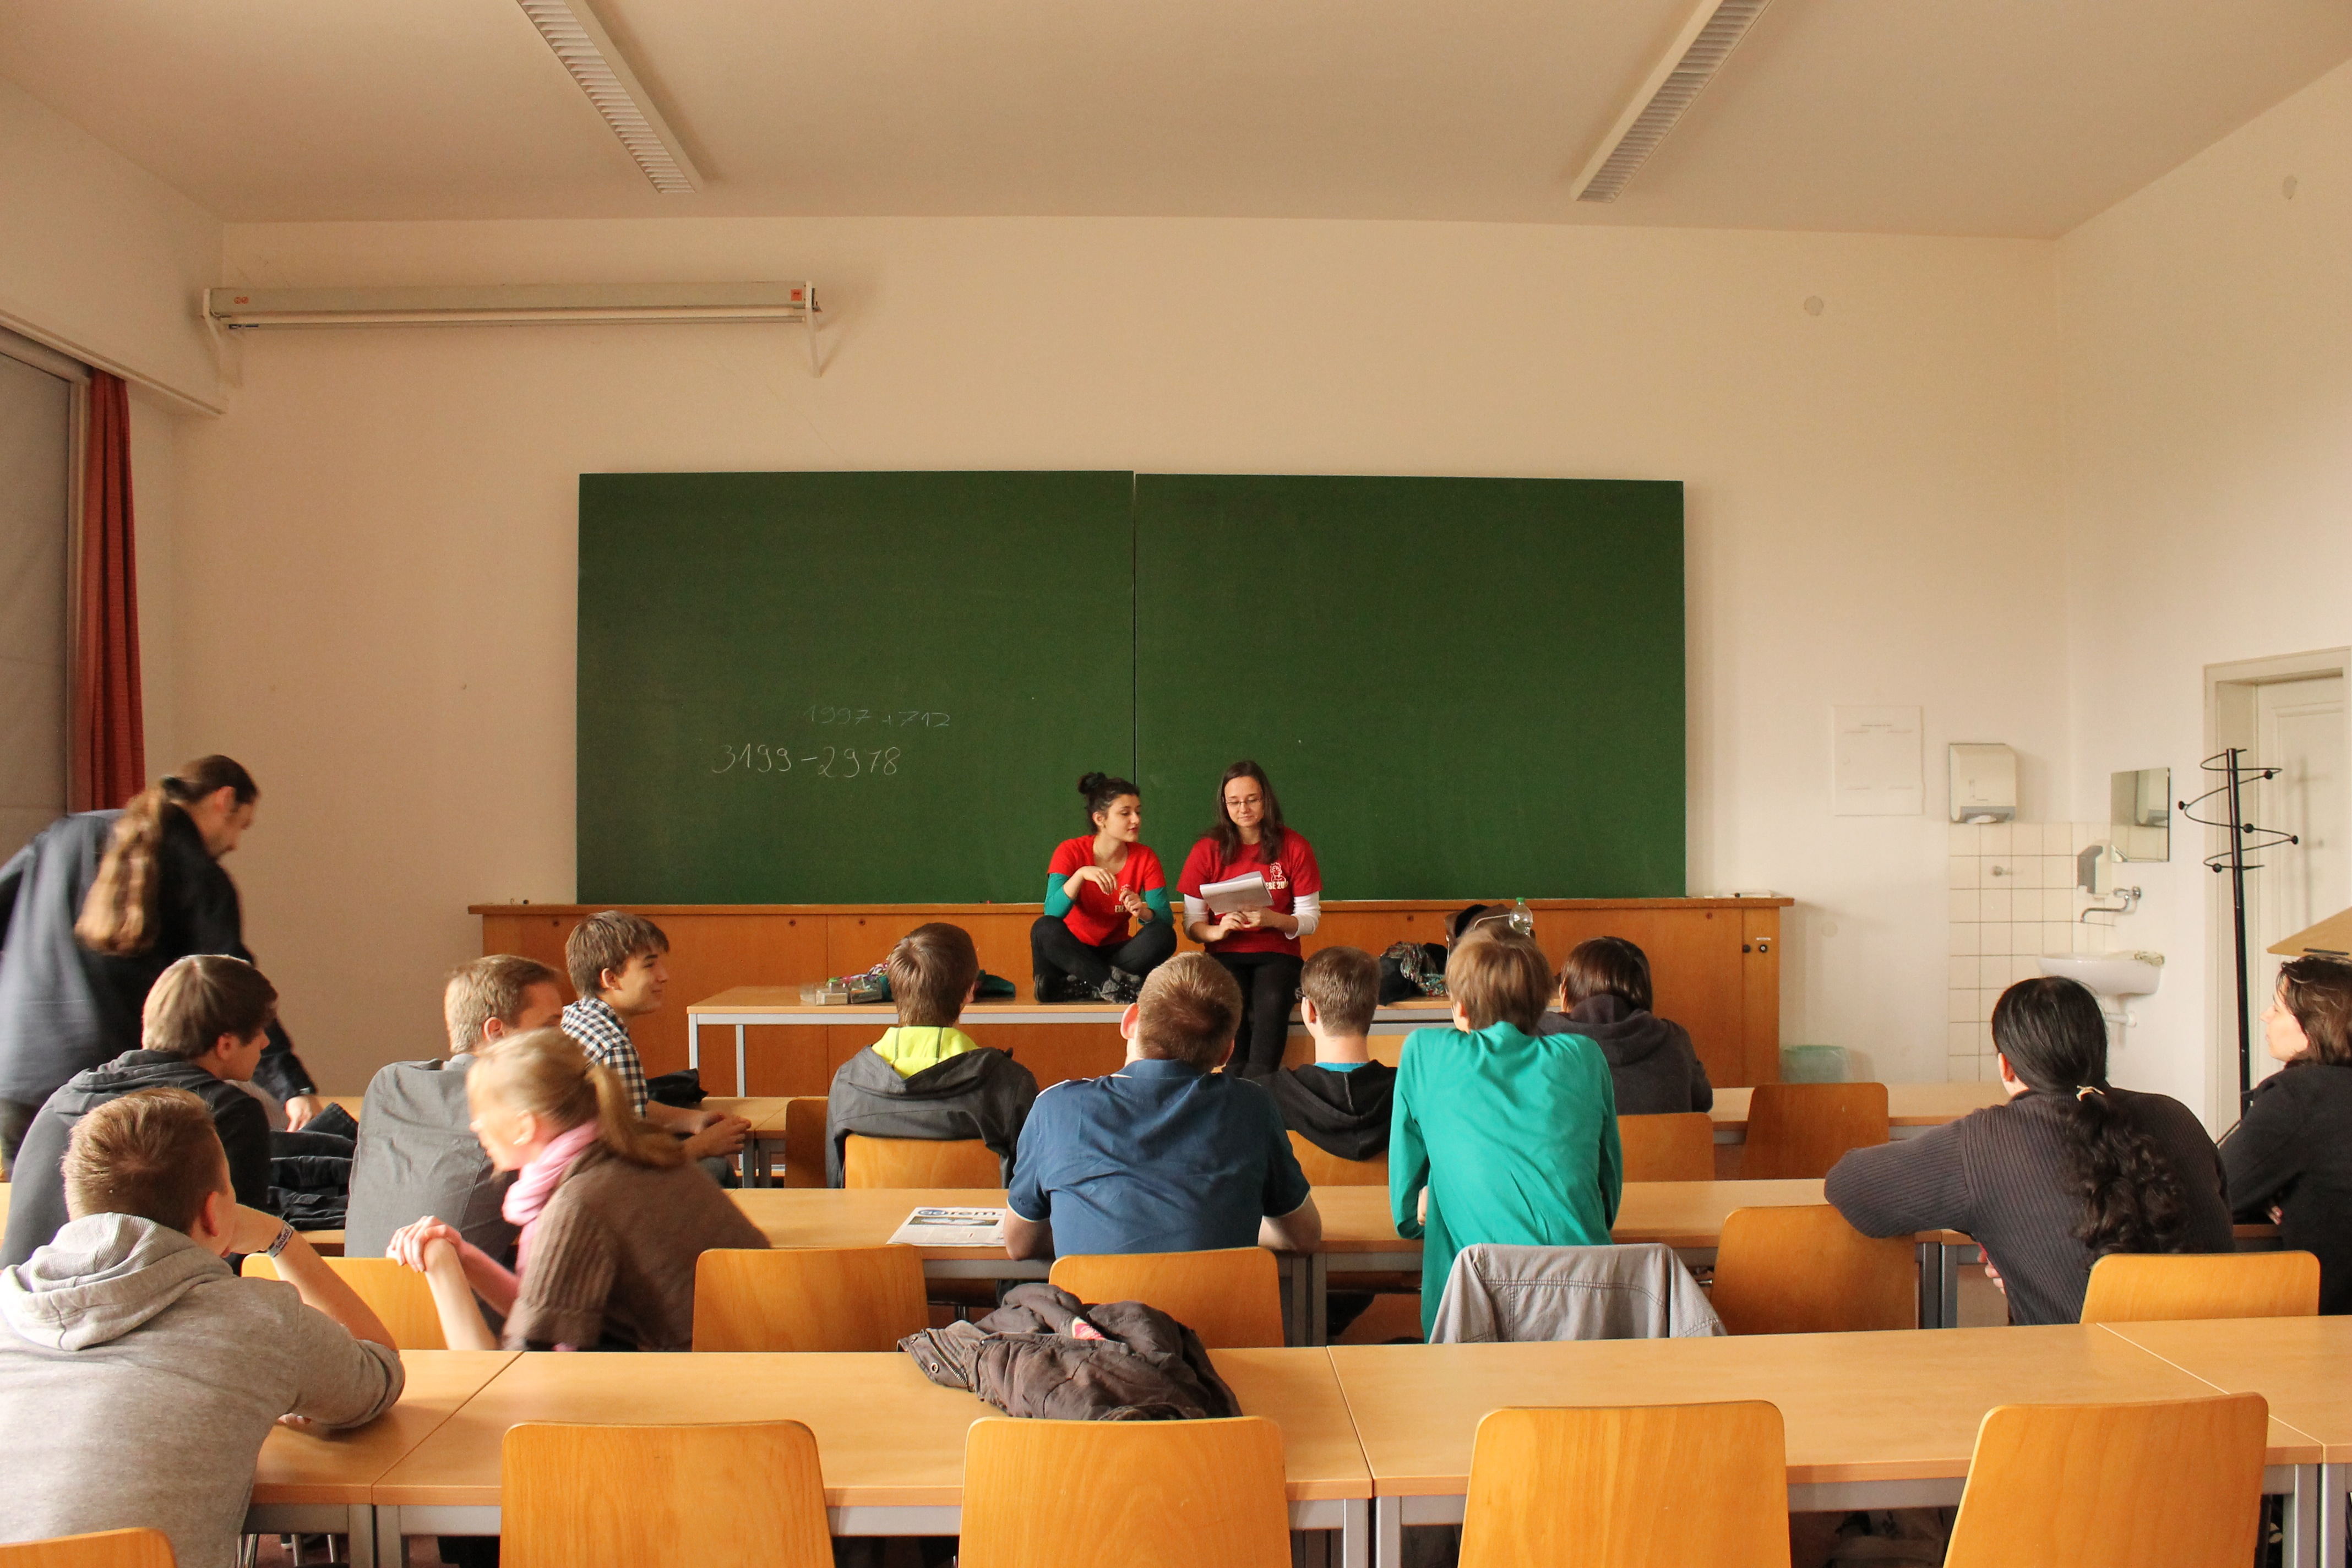
\includegraphics[width=\linewidth]{img/ese2013/tutorium.jpg}
\end{wrapfigure}

GEH WÄHLEN.
Auch wer sich nicht selbst zur Wahl aufstellen lassen will, kann was für seine Fachschaft tun.
Deine Stimme gibt dem FSR Rückhalt bei schwierigen Entscheidungen.

Wir suchen auch immer Organisationstalente für einzelne Veranstaltungen wie die Sportturniere oder die Lange Nacht der Wissenschaften.
Wenn du dich also nicht das ganze Jahr lang offiziell gewählt engagieren willst, kannst du auch als sogenanntes \textit{assoziiertes Mitglied} jederzeit mithelfen, die Rahmenbedingungen des Studiums an unserer Fakultät zu verbessern.

\textbf{Kontakt} \\
Jeden Montag trifft sich der FSR um 18:30 Uhr im großen Ratssaal (APB 1004), um unter anderem über verschiedene Aktionen, sei es ESE, Lehrevaluation, Sportturniere aber auch über Probleme und Entwicklungen an der Fakultät bzw. Universität zu diskutieren.
Du bist dabei herzlichst eingeladen, denn die Sitzung ist für alle öffentlich! Unter \link{https://www.ifsr.de/} findest du neben den Sitzungsprotokollen viele weitere nützliche Informationen.
Den Rest der Zeit sind wir eigentlich immer im Büro im Erdgeschoss des Fakultätsgebäudes (APB E017) aufzufinden.
Gerne kannst du bei Fragen auch eine E-Mail an \textit{fsr@ifsr.de} schreiben.

\minisec{auditorium}

\begin{wrapfigure}{l}{3.7cm}

\includegraphics[width=.95\linewidth]{img/auditorium_logo}
\end{wrapfigure}

Wenn du im Internet suchst, findest du nur unübersichtliche Foren?
Wikipedia kann dir auch nicht weiterhelfen?
Deinem Dozenten oder Tutor willst du keine E-Mail schreiben, weil du denkst, dass deine Frage unangebracht ist?

Keine Panik!
Wir haben die Lösung: auditorium.

Das auditorium bietet dir die Möglichkeit, Fragen zu den einzelnen Lehrveranstaltungen stellen zu können.
Diese können von deinen Kommilitonen oder den Lehrenden beantwortet, kommentiert und bewertet werden.
Wurde eine Antwort, ein Kommentar oder eine Bewertung zu deiner Frage abgegeben, wirst du darüber informiert und kannst direkt nachschauen.

Um immer die wichtigsten Fragen und Neuigkeiten zu erfahren, bietet auditorium die Möglichkeit, Lehrveranstaltungen zu verfolgen.
Folgst du einer Lehrveranstaltung, so bekommst du bei wichtigen Informationen, neuen Fragen oder Antworten eine Nachricht und weißt, was gerade wichtig ist.

{
\centering
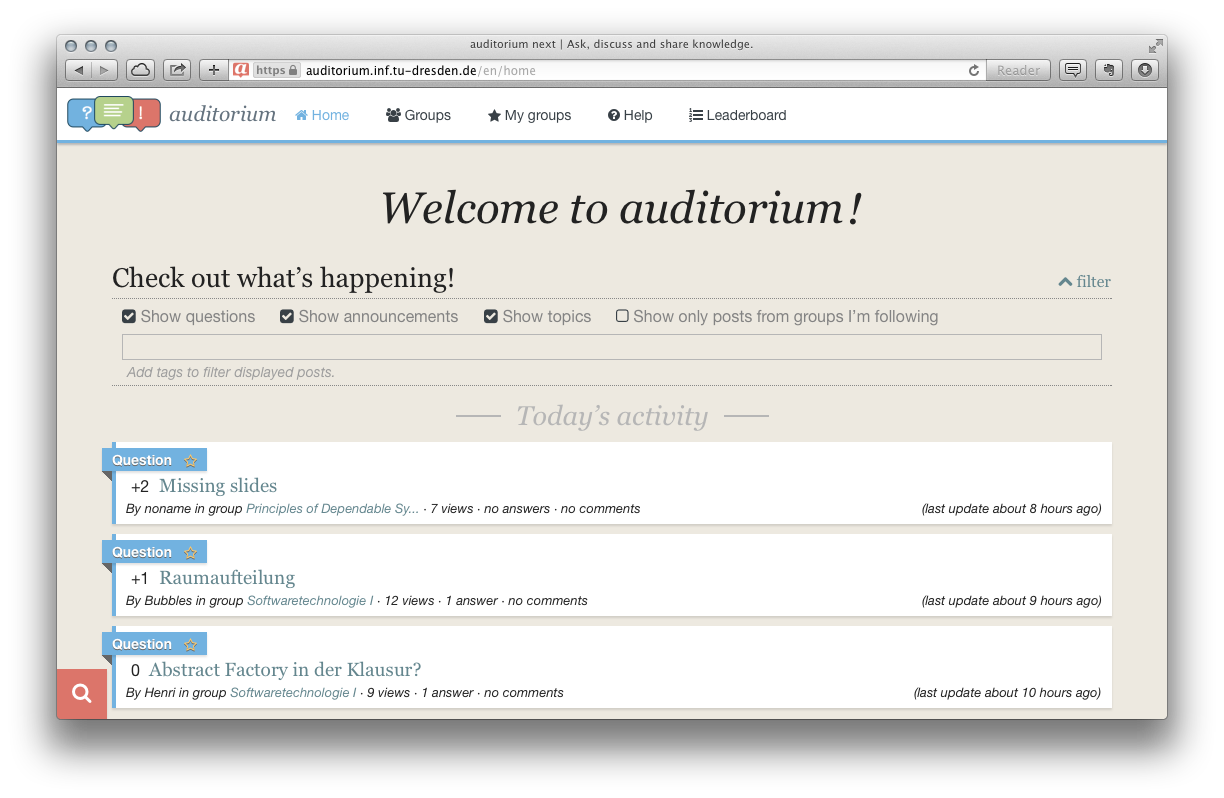
\includegraphics[width=.75\linewidth]{img/auditorium.png}
\par
}

Der Quellcode steht auf GitHub \link{https://github.com/auditorium/auditorium} zur freien Verfügung.
Jeder kann ihn dort herunterladen und selbst an der Entwicklung teilnehmen.
Falls du Fragen oder Interesse hast, dann folge uns entweder auf Twitter \textit{@\_auditorium} oder schreibe uns eine Mail an \textit{inf-auditorium@groups.tu-dresden.de}.

\newpage

\minisec{Serviceleistungen des Studentenrates (StuRa)}
Der Studentenrat ist das allen Fachschaftsräten übergeordnete Organ und vertritt die Interessen aller Studierenden der TU Dresden. Er bietet allen Studierenden eine Reihe von Serviceleistungen an:
\begin{itemize}
\item BAföG- und Sozialberatung
\item Rechtsberatung
\item Beratung für ausländische Studenten
\item Beratung für Studierende mit Kind
\item Beratung zu Anträgen und Förderungsmöglichkeiten
\item Verkauf von Karten für verschiedene Kulturveranstaltungen
\item Material- und Geräteverleih
\end{itemize}

Informationen zu allen Serviceleistungen gibt es im Studentischen Ratgeber \textit{spiritus rector} \link{http://spirex.de} und unter \link{https://www.stura.tu-dresden.de}.

\minisec{Studienberatung}
Manchmal verläuft das Studium nicht reibungslos.
Einzelne Studenten haben gerade zu Beginn des Studiums Orientierungsschwierigkeiten oder Probleme bei der Bewältigung der Anforderungen.
Die Studienberatung unterstützt dich mit Informationsangeboten in allen Phasen deines Studiums.
Die Beratung erstreckt sich beispielsweise auf Fragen zu Prüfungen und Prüfungsvorbereitung, Spezialisierungsmöglichkeiten, Studienfachwechsel oder Fragen zur Stundenplangestaltung.

Die TU Dresden bietet eine allgemeine fakultätsübergreifende Studienberatung \link{http://tu-dresden.de/studium/beratung/zentrale_studienberatung} an.

Für eine Beratung zu einem unserer beiden großen Studiengängen sind die beiden studentischen Studienberater Sascha Peukert (Informatik) und Philipp Heisig (Medieninformatik) zuständig, die gerne bei Fragen oder Problemen zur Verfügung stehen. Erreichbar sind sie unter \textit{studienberatung-inf@ifsr.de} bzw. \textit{studienberatung-minf@ifsr.de} oder gemeinsam unter \textit{studienberatung@ifsr.de}.

Darüber hinaus gibt es für jedes Studienfach einen nicht-studentischen Studienfachberater \link{https://tu-dresden.de/inf/sfb}.

\newpage

\minisec{Studentenwerk}
Das Studentenwerk betreibt nicht nur die Studentenwohnheime und versorgt die Studenten mit preisgünstiger Verpflegung in Mensen und Cafeterien, sondern bietet eine umfangreiche Betreuung und Förderung der Studenten an:
\begin{itemize}
\item Rechts- und Sozialberatung
\item Psychosoziale Beratung
\item Bearbeitung von BAföG-Anträgen
\item Bearbeitung von Anträgen auf Umzugsbeihilfe
\item Hilfestellung für Studenten mit Handicaps
\item Schwangerschaft und Kinderbetreuung im Studium
\end{itemize}
Weitere Informationen zu den Aufgaben und Angeboten des Studentenwerks findest du unter \link{https://www.studentenwerk-dresden.de/}.

\minisec{Studiendekan}
Neben dem Dekan der Fakultät und seinem Stellvertreter, dem Prodekan, gibt es noch ein weiteres Amt innerhalb der Fakultätsleitung:
den sogenannten Studiendekan.
Er ist für die Angelegenheiten der Lehre in der Fakultät zuständig, bildet den Vermittler zwischen Studenten und Professoren und hilft bei Problemen mit dem Studium allgemein.

Prof. Dr. rer. nat. habil. Weber \\
Büro: APB 1055 \\
Telefon: (0351) 463-38477 \\
E-Mail: gerhard.weber@tu-dresden.de

\minisec{Studium mit Behinderung und chronischer Krankheit}
Unter \link{https://tu-dresden.de/inf/bfsb} findest du Hilfe und Informationen, um mit Handicap im Studium gut zurecht zu kommen.

\newpage

\minisec{Prüfungsamt}
Bei Problemen mit der Prüfungseinschreibung, Notenvergabe oder jeglichen Dingen, die mit deinen Prüfungsleistungen zu tun haben, ist das Prüfungsamt der entscheidende Ansprechpartner.

Bei Fristüberschreitungen gelten Prüfungen als nicht bestanden und du könntest exmatrikuliert werden.
Unter Umständen bist du aber gar nicht schuld am Verstreichen eines Termins.
Dann solltest du einen entsprechenden Antrag an den Prüfungsausschuss (PA) stellen.
Gleiches gilt auch, wenn du eine frühere Studienleistung (also einen Leistungsnachweis oder das Ergebnis einer Prüfung) anerkannt haben möchtest.
Vorher solltet du unbedingt mit deinen zwei studentischen Vertretern im Prüfungsausschuss oder mit dem FSR sprechen.
Die Vorsitzenden der Prüfungsausschüsse sind Prof. Baier (Informatik) und Prof. Groh (Medieninformatik), in dringlichen Fällen kannst du dich direkt an sie wenden.

Wo: Prüfungsamt, APB 3039/3040 \\
Wann: Di, Do: 12.30 - 15.00 Uhr \\
Mi: 9.00 - 11.00 Uhr \\
Telefon: (0351) 463-38378

Prüfungsausschuss-Vorsitzende:

\begin{multicols}{2}
Prof. Dr. Christel Baier \\
Büro: APB 3006 \\
Telefon: (0351) 463-38548 \\
E-Mail: christel.baier@tu-dresden.de

Prof. Dr. Rainer Groh \\
Büro: APB 2065 \\
Telefon: (0351) 463-38550 \\
E-Mail: rainer.groh@tu-dresden.de
\end{multicols}

\minisec{Mund aufmachen!}
Es gibt unzählige Möglichkeiten, in brenzligen Situationen Beratung und Hilfestellung zu erhalten.
Wichtig ist nur, dass du diese bei Bedarf auch rechtzeitig in Anspruch nimmst und dich traust, bei Problemen oder Fragen die entsprechenden Stellen zu kontaktieren.
Fachliche Fragen beantworten die jeweiligen Dozenten, Kursassistenten und Tutoren immer wieder gern.
Auch kannst du dich mit anderen Studenten in Lerngruppen organisieren oder Kommilitonen älterer Semester um Hilfe bitten.
Zusätzlich steht dir innerhalb des ersten Semesters dein Seminargruppenmentor mit Rat und Tat zur Seite.
